%==================================================================%
% Author : Perez Ruiz, Alejandro                                   %
% Version: 1.0, 26/05/2011                                         %                   %                                                                  %
% Manual de ...                                                    %
%==================================================================%
\documentclass[a4paper,11pt]{article}

\usepackage[latin1]{inputenc}
\usepackage{url}
\usepackage{amsfonts}
\usepackage[spanish,activeacute]{babel}
\usepackage{graphicx}

\title{User Manual for the creation and configuration of Smart Home models}

\author{Alejandro P�rez \\ Dpto. Matem�ticas, Estad�stica y Computaci�n \\
		Universidad de Cantabria (Santander, Spain)}

\begin{document}

\maketitle

\section{Gu�a de uso para la creaci�n de modelos y configuraciones}

\subsection{Creaci�n de un nuevo proyecto para modelar y configurar hogares inteligentes y/o autom�ticos}
Para la creaci�n de un nuevo proyecto que nos permita modelar y crear configuraciones diferentes de hogares inteligentes debemos seguir los siguientes pasos:
\begin{enumerate}
\item Abrimos Visual Studio.
\item Pulsamos \emph{Archive} -->\emph{New...} --> \emph{Project}.
\item En la nueva ventana que se ha abierto seleccionamos el tipo de proyecto denominado \emph{Smart Home Project} y pulsamos sobre el bot�n \emph{OK}.
\end{enumerate}



\subsection{Modelar y crear configuraciones de hogares inteligentes y/o autom�ticos}
Para crear un modelo de un hogar inteligente y/o autom�tico debemos seguir los siguientes pasos:
\begin{enumerate}
\item A trav�s de la ventana llamada \emph{Solution Explorer} hacemos doble click sobre el archivo \emph{smartHome.sh}, que se encuentra en el proyecto \emph{MyHome}.
	\begin{center}
			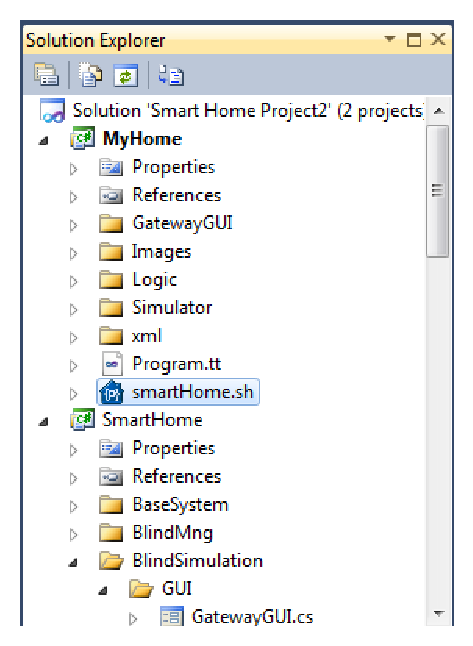
\includegraphics[width=.55\linewidth]{images/solutionExplorer.eps}
			\\
			\vspace{1cm}
	 \end{center}
\item Ahora tendremos un canvas en el que podemos arrastrar elementos. El fondo blanco representa el hogar inteligente, es decir, todo lo que arrastremos al canvas ser� una nueva caracter�stica del hogar. Para ver los elementos que pueden ser arrastrados, debemos ir a la ventana \emph{Toolbox}, sino est� visible pulsamos en \emph{View}-->\emph{Toolbox}.
	\begin{center}
			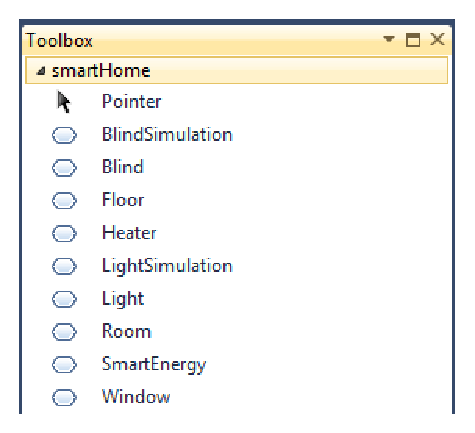
\includegraphics[width=.55\linewidth]{images/toolbox.eps}
			 \vspace{1cm}
	 \end{center}
\item Los elementos que dependen de otros, como por ejemplo las habitaciones (\emph{Room}) necesitan de una planta (\emph{Floor}), es necesario arrastrarlos encima del elemento del que dependen. De este modo, los elementos \emph{Window}, \emph{Light}, \emph{Heater}, si quieren ser a�adidos, deben ser arrastrados sobre una habitaci�n. Mientras que el elemento \emph{Blind} deber� hacerlo sobre \emph{Window}.
	 \begin{center}
			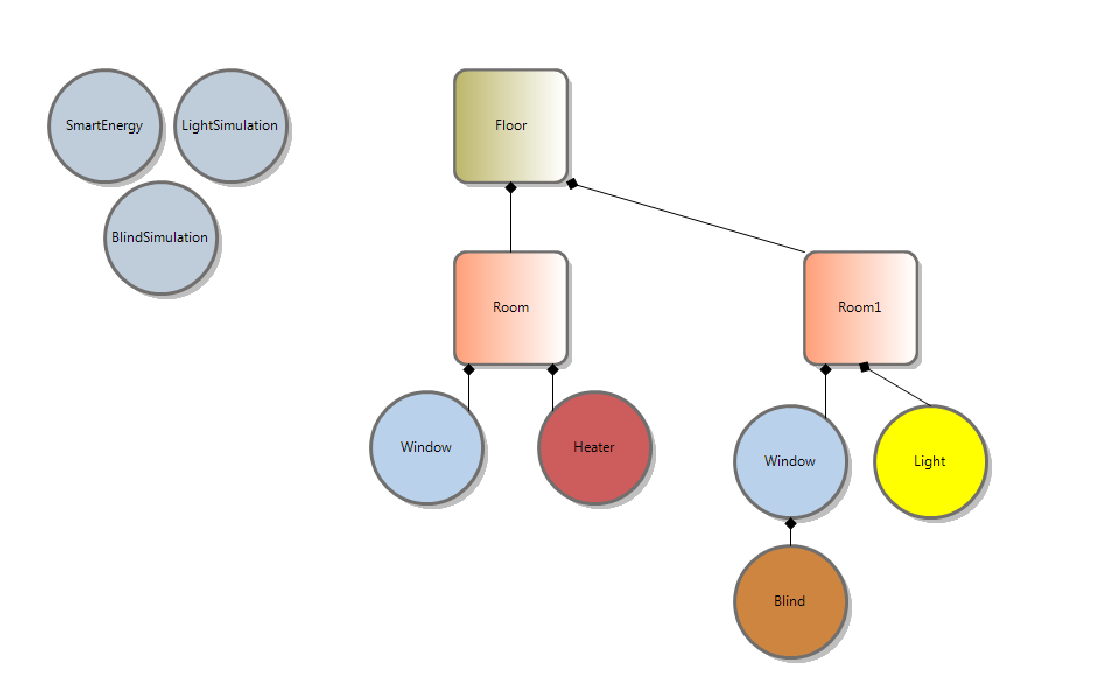
\includegraphics[width=.75\linewidth]{images/exampleSmartHome.eps}
	 \end{center}
\item Cuando tengamos el modelo preparado lo guardamos, y procedemos a generar el c�digo correspondiente para esa configuraci�n. Para ello, desde la ventana \emph{Solution Explorer}, debemos pulsar sobre el bot�n \emph{Transform All Templates}.
	\begin{center}
			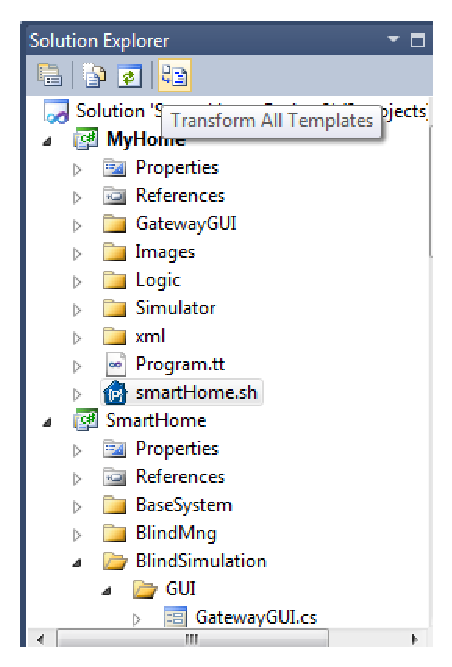
\includegraphics[width=.45\linewidth]{images/transformAllTemplates.eps}
			 \vspace{1cm}
	 \end{center}
\item Para ejecutar la configuraci�n que hemos creado, hacemos click con el bot�n derecho sobre el proyecto denominado \emph{MyHome} y escogemos \emph{Debug}-->\emph{Start New Instance}
	 \begin{center}
			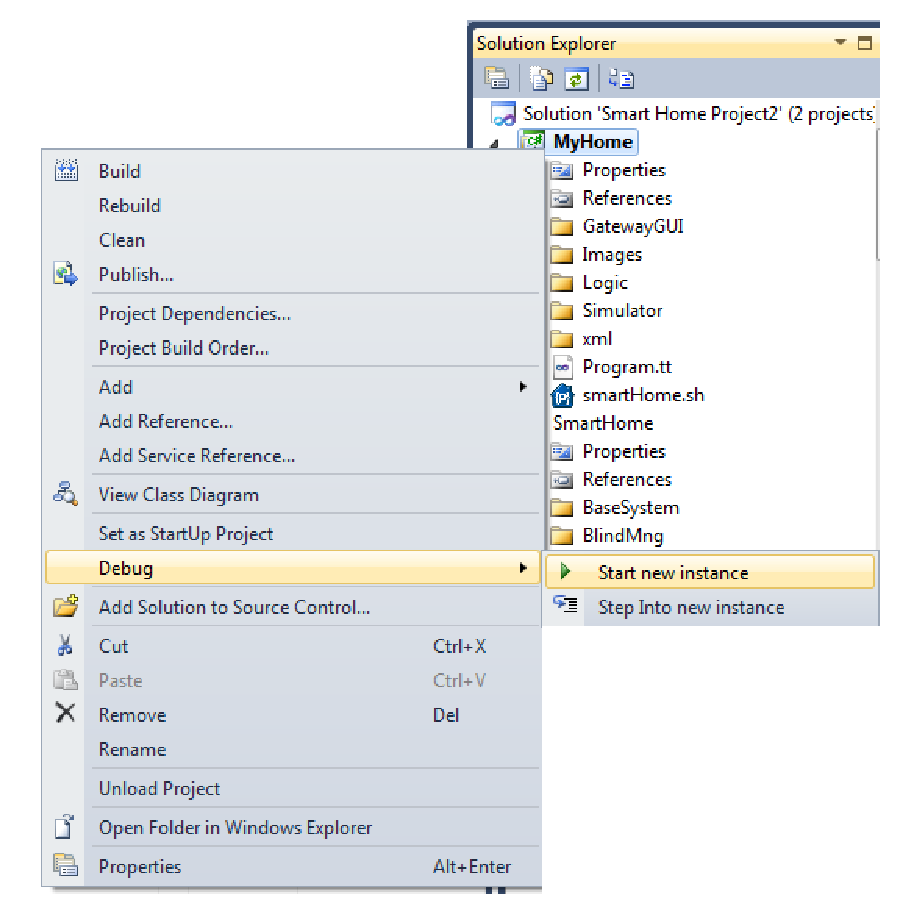
\includegraphics[width=.65\linewidth]{images/startNewInstance.eps}
			 \vspace{1cm}
	 \end{center}
\end{enumerate}

Existe la posibilidad de que cuando guardemos una configuraci�n nos alerte de alg�n error, si esto sucede, es porque hemos violado alguna de las restricciones que contiene un hogar inteligente, y se nos avisar� de ello en la ventana \emph{Error List}. Por ejemplo, si a�adimos la caracter�stica \emph{SmartEnergy}, sin que en ninguna de las habitaciones exista un calefactor y una ventana, se producir� un error por crear un modelo inv�lido.
  \begin{center}
			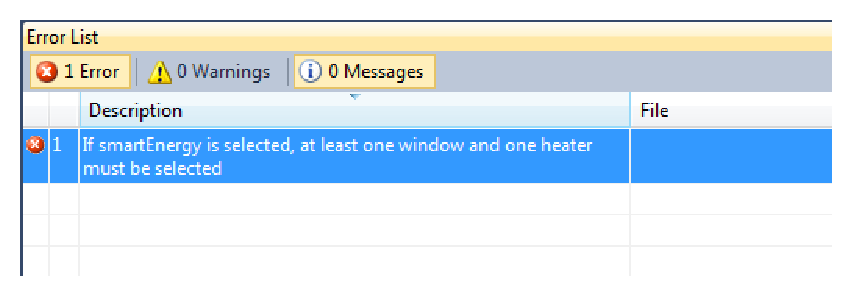
\includegraphics[width=.55\linewidth]{images/error.eps}
			 \vspace{1cm}
  \end{center}

\end{document}
